% file: EM_dump.tex
% Electrodynamics, in unconventional ``grande'' format; fitting a widescreen format
% Electricity and Magnetism notes "dump" 
% 
% github        : ernestyalumni
% linkedin      : ernestyalumni 
% wordpress.com : ernestyalumni
%
% This code is open-source, governed by the Creative Common license.  Use of this code is governed by the Caltech Honor Code: ``No member of the Caltech community shall take unfair advantage of any other member of the Caltech community.'' 
% 

\documentclass[10pt]{amsart}
\pdfoutput=1
\usepackage{mathtools,amssymb,lipsum,caption}

\usepackage{graphicx}
\usepackage{hyperref}
\usepackage[utf8]{inputenc}
\usepackage{listings}
\usepackage[table]{xcolor}
\usepackage{pdfpages}
%\usepackage[version=3]{mhchem}
\usepackage{mhchem}

\usepackage{tikz}
\usetikzlibrary{matrix,arrows}

\usepackage{multicol}

\hypersetup{colorlinks=true,citecolor=[rgb]{0,0.4,0}}

\oddsidemargin=15pt
\evensidemargin=5pt
\hoffset-45pt
\voffset-55pt
\topmargin=-4pt
\headsep=5pt
\textwidth=1120pt
\textheight=595pt
\paperwidth=1200pt
\paperheight=700pt
\footskip=40pt


\newtheorem{theorem}{Theorem}
\newtheorem{corollary}{Corollary}
%\newtheorem*{main}{Main Theorem}
\newtheorem{lemma}{Lemma}
\newtheorem{proposition}{Proposition}

\newtheorem{definition}{Definition}
\newtheorem{remark}{Remark}

\newenvironment{claim}[1]{\par\noindent\underline{Claim:}\space#1}{}
\newenvironment{claimproof}[1]{\par\noindent\underline{Proof:}\space#1}{\hfill $\blacksquare$}

%This defines a new command \questionhead which takes one argument and
%prints out Question #. with some space.
\newcommand{\questionhead}[1]
  {\bigskip\bigskip
   \noindent{\small\bf Question #1.}
   \bigskip}

\newcommand{\problemhead}[1]
  {
   \noindent{\small\bf Problem #1.}
   }

\newcommand{\exercisehead}[1]
  { \smallskip
   \noindent{\small\bf Exercise #1.}
  }

\newcommand{\solutionhead}[1]
  {
   \noindent{\small\bf Solution #1.}
   }


\title{Electromagnetism, Electrodynamics Dump;  \large Electricity and Magnetism dump (includes notes and solutions to Purcell's Electricity and Magnetism}
\author{Ernest Yeung \href{mailto:ernestyalumni@gmail.com}{ernestyalumni@gmail.com}}
\date{7 mars 2017}
\keywords{Electromagnetism, Electrodynamics, Electricity, Magnetism}
\begin{document}

\definecolor{darkgreen}{rgb}{0,0.4,0}
\lstset{language=Python,
 frame=bottomline,
 basicstyle=\scriptsize,
 identifierstyle=\color{blue},
 keywordstyle=\bfseries,
 commentstyle=\color{darkgreen},
 stringstyle=\color{red},
 }
%\lstlistoflistings

\maketitle

From the beginning of 2016, I decided to cease all explicit crowdfunding for any of my materials on physics, math.  I failed to raise \emph{any} funds from previous crowdfunding efforts.  I decided that if I was going to live in \emph{abundance}, I must lose a scarcity attitude.  I am committed to keeping all of my material \textbf{open-sourced}.  I give all my stuff \emph{for free}.   

In the beginning of 2017, I received a very generous donation from a reader from Norway who found these notes useful, through \emph{PayPal}.  If you find these notes useful, feel free to donate directly and easily through Venmo (@ernestyalumni) or Cash App (\$Ernesttravels), which won't go through a 3rd. party such as indiegogo, kickstarter, patreon.  Otherwise, under the \emph{open-source MIT license}, feel free to copy, edit, paste, make your own versions, share, use as you wish.

\noindent gmail        : ernestyalumni \\
linkedin     : ernestyalumni \\
twitter      : ernestyalumni \\


  
\setcounter{tocdepth}{1}
\tableofcontents

\begin{multicols*}{2}


\begin{abstract}
Electricity and Magnetism notes "dump" - Everything about or involving electricity and magnetism, electrodynamics.

\end{abstract}

\part{Math}

\section{Codifferential, The "Vector Potential" and Laplacian}  
\emph{Keywords}: codifferential, vector potential, Laplacian

\subsection{Codifferential $\delta$}

For smooth manifold $M$, $\text{dim}M = n$, 
\begin{equation}
\boxed{
\begin{aligned}
	& \delta : \Omega^k(M) \to \Omega^{k-1}(M) \\ 	
	& \delta = (-1)^{n(k+1)+1} * d*
\end{aligned}
}
\end{equation}

For $k=1,2$ cases, 
\[
\begin{aligned}
	& \delta = (-1)^{n(1+1)+1} * d* = (-1) *d* \\ 
	& \delta = (-1)^{n(2+1) + 1} * d * = (-1)^{3n+1} *d*
\end{aligned}
\]
For $n=d=3$, 
\[
\begin{aligned}
	& \mathbf{\delta} : \Omega^2(M) \to \Omega^1(M) \\ 
	& \mathbf{\delta} = \mathbf{* d * }
\end{aligned}
\]

\subsection{the "Vector Potential"}

If $B=\mathbf{d} A$, $B\in \Omega^2(M)$, 
\[
\begin{gathered}
B= B_{jk} dx^j \wedge dx^k = \mathbf{d}A = \frac{ \partial A_k}{ \partial x^j} dx^j \wedge dx^k  \\
 B_{jk} = \frac{ \partial A_k}{ \partial x^j} 
\end{gathered}
\]
So these statements are equivalent: 
\begin{equation}
\boxed{ 
B =\mathbf{d} A \Longleftrightarrow \mathbf{B} = \text{curl} \mathbf{A}
}
\end{equation}

Indeed, recall the \emph{deRham cohomology}:

\[
\begin{gathered}
	H^k_{\text{deRham}}(M) = Z^k(M)/ \text{im}d = \frac{Z^k(M)}{ d\Omega^{k-1}(M) }
\end{gathered}
\]
And so this form for $B=\mathbf{d}A$ presupposes that 
\[
B \in [1] = [\mathbf{d}A ] \in H^2_{\text{deRham}}(M')
\]
But it should be noted on another manifold, this form may not hold; indeed, consider a submanifold or domain $M' \subseteq M$.  In this case
\[
H^2_{\text{deRham}}(M') \ni B
\]

\subsection{Laplacian}

\begin{definition}[Laplacian]
\begin{equation}
\begin{aligned}
	& \Delta : \Omega^k(M) \to \Omega^k(M) \\ 
	& \Delta = d\delta + \delta d
\end{aligned}
\end{equation}
\end{definition}

Both recognizing the equivalence between these 2 formulations:
\[
\mathbf{*d*}B = \mathbf{\delta}B \Longleftrightarrow \text{curl} \mathbf{B}
\]
and acknowledging that it \emph{has} to be the case that $\mathbf{*d*}B$ is the correct expression, coming from $d*F$ for the electromagnetic 2-form $F$, 
\[
\mathbf{\delta} B = \mathbf{\delta} \mathbf{d}A = \Delta A - \mathbf{d \delta} A
\]
Then
\[
\begin{gathered}
	\mathbf{*d}A = \frac{ \sqrt{|\mathbf{g} |} }{ (d-2)! } \epsilon_{i_1i_2 \dots i_{d-2} jk} g^{jj'} g^{kk'} \frac{ \partial A_{k'}}{ dx^{j'} } dx^{i_1} \wedge \dots \wedge dx^{i_{d-2}} = \sqrt{ |\mathbf{g} | } \epsilon_{ijk} g^{jj'} g^{kk'} \frac{ \partial A_{k'} }{ \partial x^{j'} } dx^i  \\
\end{gathered}
\]


Consider the expression 
\[
\text{curl}\mathbf{B} = \text{curl}( \text{curl} \mathbf{A})
\]
I will generalize it and point out its misgivings.  

Calculating from definitions for $*$ and $d$, 
\[
\begin{gathered}
	\mathbf{d} \mathbf{*} \mathbf{d} A = \frac{ \epsilon_{i_1 i_2 \dots i_{d-2} jk } }{ (d-2)! } \frac{ \partial }{ \partial x^l} \left( \sqrt{|\mathbf{g} |} g^{jj'} g^{kk'} \frac{ \partial A_{k'} }{ \partial x^{j'} } \right) dx^l \wedge dx^{i_1} \wedge \dots \wedge dx^{i_{d-2} } \\ 
	\mathbf{*} \mathbf{d} \mathbf{*} \mathbf{d} A = \frac{ \sqrt{ |\mathbf{g} | } }{ (d-d(-1))! } \frac{ \epsilon_{id'i_1' i_2' \dots i'_{d-2} } }{ (d-2)! } g^{l'l} g^{i_1' i_1} g^{i_2' i_2} \dots g^{i_{d-2}' i_{d-2} } \frac{ \partial }{ \partial x^l } \left( \sqrt{ |\mathbf{g} | } g^{jj'} g^{kk'} \frac{ \partial A_{k'} }{ \partial x^{j'} } \right) \epsilon_{i_1 i_2 \dots i_{d-2} jk } dx^i = \\
\xrightarrow{d=3} \sqrt{ |\mathbf{g} | } \epsilon_{il'm'} g^{l'l} g^{m'm} \frac{ \partial }{ \partial x^l} \left( \sqrt{ |\mathbf{g} | } g^{jj'} g^{kk'} \frac{ \partial A_{k'} }{ \partial x^{j'} } \right) \epsilon_{mjk} dx^i
\end{gathered}
\]
In $\mathbb{R}^3$, 
\[
\mathbf{*} \mathbf{d} \mathbf{*} \mathbf{d} A \xrightarrow{ \mathbb{R}^3} \frac{ \partial }{ \partial x^j} \left( \frac{ \partial A_k }{ \partial x^j} \right) - \frac{ \partial }{ \partial x^k} \left( \frac{ \partial A_k}{ \partial x^j} \right)
\]
At this point, in the "vector calculus" formulation, the partial derivatives in the $- \frac{ \partial }{ \partial x^k} \left( \frac{ \partial A_k}{ \partial x^j} \right)$ would be exchanged in order, and then a so-called "choice of gauge" for $\nabla \cdot A \equiv \text{div}A$ would be "made," making this term equal $0$.  As we clearly see above, this should not be the case.  Rather, this choice should be made:
\begin{equation}
\mathbf{d \delta } A = 0
\end{equation}
This is because we should directly use the "manifestly covariant" definition of the Laplacian:
\begin{equation}
\begin{gathered}
	\mathbf{* d * d } A = (-1)^{d(1-1) +1} \mathbf{ \delta d} A = (-1)^{0+1} \mathbf{ \delta d } A = (-1)^{1} (\Delta - \mathbf{d\delta } ) A \\
\xrightarrow{ d=3} (-1)(\Delta - \mathbf{ d\delta } ) A	
\end{gathered}
\end{equation}
Note that $k=1$, i.e. we're dealing with 1-form $A$ here, in the $(-1)^{d(k-1)+1}$ factor.  

So the true expression is this (to reiterate and emphasize the point):
\begin{equation}	
\mathbf{\delta}B = (-1) (\Delta - \mathbf{d\delta } ) A
\end{equation}

Are there any necessary constraints on $A$ to make it, such that $\mathbf{d\delta }A=0$?  Perhaps we can take a look at how the definition of the codifferential $\mathbf{\delta}$ necessitates that this diagram commutes:
\[
 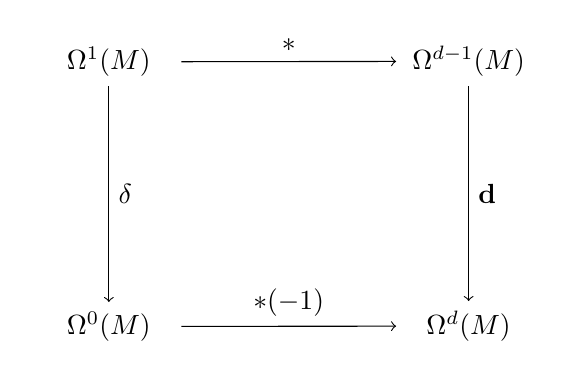
\begin{tikzpicture}
  \matrix (m) [matrix of math nodes, row sep=7.8em, column sep=7.8em, minimum width=5.2em]
  {
 \Omega^1(M)  &  \Omega^{d-1}(M)  \\ 
	\Omega^0(M) &  \Omega^d(M)  \\ 
};
  \path[->]
  (m-1-1) edge node [above] {$ \mathbf{*} $ }  (m-1-2)
edge node [auto] {$\mathbf{\delta} $ } (m-2-1) 
	(m-1-2) edge node [auto] {$ \mathbf{d} $ } (m-2-2)
	(m-2-1) edge node [auto] {$ \mathbf{ * } (-1) $ }(m-2-2)
  ;
\end{tikzpicture}   \qquad \quad \, 
\begin{tikzpicture}
  \matrix (m) [matrix of math nodes, row sep=7.8em, column sep=7.8em, minimum width=5.2em]
  {
 A  &  \mathbf{*}A  \\ 
	\delta A &  \mathbf{d}\mathbf{*} A  \\ 
};
  \path[|->]
  (m-1-1) edge node [above] {$ \mathbf{*} $ }  (m-1-2)
edge node [auto] {$\mathbf{\delta} $ } (m-2-1) 
	(m-1-2) edge node [auto] {$ \mathbf{d} $ } (m-2-2)
	(m-2-1) edge node [auto] {$ \mathbf{ * } (-1) $ }(m-2-2)
  ;
\end{tikzpicture}  
\]

\part{Electrostatics}



\part{Maxwell's Equations; My version of Maxwell's Equations}

\section{My version of Maxwell's equations}

\subsection{Maxwell's Equations, my version, in "vector calculus" form}

If $\nabla \cdot \mathbf{B} = 0$, then
\begin{equation}
	\nabla \times \mathbf{E} = \frac{-1}{c} \left( \frac{ \partial \mathbf{B} }{\partial t} \right)
\end{equation}

If $\nabla \cdot \mathbf{E} = 4\pi \rho_{\text{total}}$, then 
\begin{equation}
\begin{aligned}
	\nabla \times \mathbf{B} & = \frac{1}{c} \left( \frac{ \partial \mathbf{E}}{ \partial t} + 4\pi \frac{ \partial \mathbf{P} }{ \partial t} +  \right.  \\
	& \left.   + 4\pi \mathbf{J}_{\text{free}} + 4\pi c \nabla \times \mathbf{M}  \right)
\end{aligned}
\end{equation}

\subsection{Maxwell's Equations, my version, over spacetime manifold $M$}

For spacetime manifold $M$, of dimensions $\text{dim}M = d+1$, and for 
\[
\begin{aligned}
	& E \in \Omega^1(M) \\ 
	& B \in \Omega^2(M)
\end{aligned}
\]
If $\mathbf{d}B=0$, then 
\begin{equation}\label{Eq:MaxwellsEqnsDGEBInduction}
\boxed{ 	\mathbf{d}E + \frac{ \partial B}{ \partial t} = 0  }
\end{equation}

If $\mathbf{\delta}E = \mathbf{*} \mathbf{d} \mathbf{*} E = 4\pi \rho_{\text{total}}$, 
\begin{equation}\label{Eq:MaxwellsEqnsDGEBFaraday}
	\boxed{ \mathbf{\delta} B = \mathbf{*} \mathbf{d} \mathbf{*} B = \frac{ \partial E}{ \partial t} + 4\pi \frac{ \partial P}{ \partial t} + 4\pi J_{\text{free}} + 4\pi c \mathbf{\delta} \mathbf{M} }
\end{equation}
with $\mathbf{M} \in \Omega^2(M)$, magnetization in matter (i.e. matter magnetization) is \emph{necessarily} a 2-form.  

\subsubsection{Some of the algebra (scratch) work/explicit calculations, for Maxwell's Equations, my version, over spacetime manifold $M$}

\[
\mathbf{d}B \Longleftrightarrow \nabla \cdot B
\]
since component-wise, 
\[
\begin{gathered}
	\mathbf{d} B = \frac{ \partial }{ \partial x^k } B_{ij} dx^k \wedge dx^i \wedge dx^j \Longleftrightarrow \nabla \cdot B 
\end{gathered}
\]
\[
\mathbf{d}E = -\frac{ \partial B}{\partial t}   \Longleftrightarrow \nabla \times E \equiv \text{curl} E = \frac{-1}{c} \frac{ \partial \mathbf{B}}{ \partial t}  
\]
since, component-wise, 
\[
\mathbf{d} E = \frac{ \partial }{ \partial x^k} E_i dx^k \wedge dx^i = \frac{ \partial }{ \partial x^j} E_k dx^j \wedge dx^k = \frac{ -\partial }{ \partial t} B_{jk} dx^j \wedge dx^k 
\]
For $\mathbf{\delta} E = \mathbf{*} \mathbf{d} \mathbf{*} E = 4\pi \rho_{\text{total}}$, consider
\[
\begin{gathered}
	\mathbf{*} E = \frac{1}{ (d-1)!} \sqrt{ \mathbf{g}} \epsilon_{i_1i_2 \dots i_{d-1} j_1} E_j g^{jj_1} e^{i_1} \wedge e^{i_2} \wedge \dots \wedge e^{i_{d-1}} = \frac{1}{2} \sqrt{ \mathbf{g}} \epsilon_{ijk} E_{k'} g^{k'k} dx^i \wedge dx^j 
\end{gathered}
\]
Further, 
\[
\begin{gathered}
	\mathbf{d} \mathbf{*} E = \frac{1}{ (d-1)! } \frac{ \partial }{ \partial x^k} (\sqrt{ \mathbf{g}} E_j g^{jj_1} ) \epsilon_{i_1 i_2 \dots i_{d-1} j_1 } dx^k \wedge dx^{i_1} \wedge dx^{i_2} \wedge \dots \wedge dx^{i_{d-1}} = \\
=\frac{1}{(d-1)!} \frac{ \partial }{ \partial x^k} (\sqrt{ \mathbf{g}} E^{j_1} ) \epsilon_{i_1 i_2 \dots i_{d-1} j_1} \epsilon^{ k i_1 i_2 \dots i_{d-1} } \frac{ \text{vol}^d}{ \sqrt{ |\mathbf{g} | } } = \\
=\frac{1}{(d-1)!} \frac{ \partial }{ \partial x^k} (\sqrt{ |\mathbf{g} | } E^{j_1} ) \delta^k_{ j_1} (d-1)! \frac{ \text{vol}^d}{ \sqrt{ |\mathbf{g} | } } = \frac{1}{ \sqrt{ |\mathbf{g} | }} \frac{ \partial }{ \partial x^k} (\sqrt{ |\mathbf{g} |} E^k) \text{vol}^d 
\end{gathered}
\]
where this (generalized) Kronecker delta relation was used: 
\[
\frac{1}{p!} \delta^{\mu_1 \dots \mu_p }_{\nu_1 \dots \nu_p } \delta^{ \nu_1 \dots \nu_p }{ \rho_1 \dots \rho_p } = \delta^{\mu_1 \dots \mu_p }_{ \rho_1 \dots \rho_p }
\]
where 
\[
\delta^{\mu_1 \dots \mu_n }_{ \nu_1 \dots \nu_n } = \epsilon^{\mu_1 \dots \mu_n} \epsilon_{ \nu_1 \dots \nu_n }
\]
Note that 
\[
\begin{aligned}
	*1 & = \text{vol} \\
**1  & = (-1)^{0(n-0)} 1 = 1 = *\text{vol}
\end{aligned}
\]
and so 
\[
\mathbf{*} \mathbf{d} \mathbf{*} E = \mathbf{\delta} E = \frac{1}{\sqrt{ |\mathbf{g} | } } \frac{ \partial }{ \partial x^k} ( \sqrt{ | \mathbf{g} | } E^k )
\]
Indeed, we had generalized the divergence, but on a 1-form:
\begin{equation}
\begin{aligned}
	& \mathbf{\delta} : \Omega^1(M) \to C^{\infty}(M) \\ 
	& -\mathbf{\delta} E = -\mathbf{\delta} (E_kdx^k)  = \frac{1}{\sqrt{|\mathbf{g} |} } \frac{ \partial }{ \partial x^k} (\sqrt{ |\mathbf{g} | } E^k) \equiv \frac{1}{\sqrt{ |\mathbf{g} | } } \frac{ \partial }{ \partial x^k} ( \sqrt{ |\mathbf{g} | }  g^{kk_1} E_{k_1} )
\end{aligned}
\end{equation}

\section{Magnetostatics, macroscopic Magnetism, Magnetic permeability, magnetic susceptibility, field $\mathbf{H}$, free currents and field $\mathbf{H}$}

\emph{Keywords}: magnetic permeability, magnetic susceptibility

Suppose we have matter (i.e. the "macroscopic problem", referred to from Jackson (1998), Sec. 5.8 "Macroscopic Equations, Boundary Conditions on $B$ and $H$", \cite{Jack1998}), \emph{not} a vacuum.  

Atoms in matter have electrons, $e^-$ in orbit, contributing to (rapidly) fluctuating magnetic moments $\mathbf{m}$, along with $e^-$'s intrinsic $\mathbf{m}$.  

Consider an average macroscopic magnetization or magnetic moment density $\mathbf{M}(\mathbf{x})$ defined in a "vector calculus" manner by Jackson (1998) \cite{Jack1998}, 
\[
\mathbf{M}(\mathbf{x}) = \sum_I N_I\langle \mathbf{m}_I\rangle , \qquad \, I \equiv \text{ index of a particle } 
\]

Recalling Maxwell's Equations, Eq. \ref{Eq:MaxwellsEqnsDGEBFaraday}, 
\[
\mathbf{\delta} B = \frac{ \partial E}{ \partial t} + 4\pi \frac{ \partial P }{ \partial t} + 4\pi J_{\text{free}} + 4\pi c \mathbf{\delta}\mathbf{M}
\]
Consider a time-independent $E$ and negligible $P$.  Then 
\[
\Longrightarrow \mathbf{\delta} B =  4\pi J_{\text{free}} + 4\pi c \mathbf{\delta}\mathbf{M}
\]
Jackson (1998) \cite{Jack1998} considers this magnetization $\mathbf{M}$ as contributing to an \emph{effective current density} by vector calculus arguments of it having a vector potential form, and so he proceeds to write it as (Jackson (1998), Eqn. (5.80) \cite{Jack1998})
\[
\text{curl} \mathbf{B} = \mu_0 (\mathbf{J} + \text{curl}\mathbf{M} ) \qquad \, (SI)
\]
Then Jackson \emph{defines} the macroscopic field $\mathbf{H}$, in Jackson (1998), Eqn. (5.81) \cite{Jack1998}, 
\[
\mathbf{H} := \frac{1}{\mu_0} \mathbf{B} - \mathbf{M}
\]

However, Purcell's treatment is both more lucid, and more grounded in what $B$ field really is physically, less relying upon artificial artifices.  

\subsection{Free currents $\mathbf{J}_{\text{free}}$ and the field $\mathbf{H}$, magnetic susceptibility}

cf. Purcell (1984) \cite{Purc1984}, Sec. 11.10 Free Currents, and the Field $\mathbf{H}$  

\emph{Keywords}: $\mathbf{H}$, volume magnetic susceptibility

Bound current $\mathbf{J}_{\text{bound}}$ are current associated with molecular or atomic magnetic moments, including the intrinsic magnetic moment of particles with spin.  

Free currents $\mathbf{J}_{\text{free}}$ are ordinary conduction currents.  

\begin{equation}
\mathbf{J}_{\text{bound}} = c \nabla \times \mathbf{M}
\end{equation}
cf. Purcell (1984), Eq. (44) of Ch. 11 \cite{Purc1984}

At a surface, where $\mathbf{M}$ is discontinuous, we have a surface current density $\mathcal{J}$.  


By superposition, 
\begin{equation}
	\nabla \times \mathbf{B} = \frac{ 4\pi }{c} (\mathbf{J}_{\text{bound}} + \mathbf{J}_{\text{free} } ) = \frac{4\pi }{ c} \mathbf{J}_{\text{total} }
\end{equation}
cf. Purcell (1984), Eq. (50) of Ch. 11 \cite{Purc1984}

Thus, 
\[
\begin{gathered}
\nabla \times \mathbf{B} = \frac{ 4\pi}{c}(c\nabla \times \mathbf{M} ) + \frac{4\pi}{c} \mathbf{J}_{\text{free}} = \\
	= \nabla \times (\mathbf{B} - 4\pi \mathbf{M} ) = \frac{4\pi }{c} \mathbf{J}_{\text{free} }
\end{gathered}
\]
cf. Purcell (1984), Eq. (51) of Ch. 11 \cite{Purc1984}

Purcell also defines 
\begin{equation}
\mathbf{H} := \mathbf{B}-4\pi \mathbf{M}
\end{equation}
cf. Purcell (1984), Eq. (52) of Ch. 11 \cite{Purc1984}; and so 
\[
\begin{gathered}
\nabla \times \mathbf{H} = \frac{4\pi}{c} \mathbf{J}_{\text{free}} \qquad \, (cgs) \qquad \qquad \, \nabla \times \mathbf{H} = \mathbf{J}_{\text{free}} \qquad \, (SI)
\end{gathered}
\]
cf. Purcell (1984), Eq. (53), (53'), respectively, of Ch. 11 \cite{Purc1984}.  

In magnetic systems, it is precisely the free currents that we can control.  So $\mathbf{H}$ is useful:

\begin{equation}
\begin{gathered}
\int_C \mathbf{H} \cdot d\mathbf{l} = \frac{4\pi}{c}\int_S \mathbf{J}_{\text{free}} \cdot d\mathbf{a} = \frac{4\pi}{c} I_{\text{free}} \qquad \, (cgs) \qquad \qquad \, \int_C \mathbf{H} \cdot d\mathbf{l} = \int_S \mathbf{J}_{\text{free}} \cdot d\mathbf{a} =  I_{\text{free}} \qquad \, (SI)
\end{gathered}
\end{equation}
where in SI, $H \sim \frac{ \text{ amps } }{ \text{ meter } }$.  cf. Purcell (1984), Eq. (54), (54'), respectively, of Ch. 11 \cite{Purc1984}.  

$\mathbf{B}$ is the \emph{fundamental magnetic field vector}; it is \textbf{only} $\mathbf{B}$ s.t. $\nabla \cdot \mathbf{B} =0$ or $\mathbf{d}B=0$  

The basic magnetic field inside matter is $\mathbf{B}$, \emph{not} $\mathbf{H}$.  That's not a matter of mere definition, but a \emph{consequence of the absence of magnetic charges}.  cf. Purcell (1984)\cite{Purc1984}.   

Now 
\begin{equation}
\mathbf{M} = \chi_m \mathbf{H}
\end{equation}
cf. Purcell (1984), Eq. (56) Ch. 11 \cite{Purc1984}. 

The lines of $\mathbf{H}$ inside the magnet look just like the lines of $\mathbf{E}$ inside the polarized cylinder.   \\
- $\mathbf{H}$ is the fiction of magnetic poles; if there wre magnetic poles then $\mathbf{H}$ is the macroscopic $\mathbf{B}$ filed inside the material.  

For any material in which $\mathbf{M}$ is porportional to $\mathbf{H}$, 
\begin{equation}
\boxed{ 
\begin{gathered}
	\mathbf{B} = \mathbf{H} + 4\pi \mathbf{M} = (1+4\pi \chi_m) \mathbf{H} \\
\mu = 1 + 4\pi \chi_m
\end{gathered}
}
\end{equation}

So \emph{if} there was a linear response between magnetization $\mathbf{M}$ and the measured macroscopic field $\mathbf{H}$, related through the volume magnetic susceptibility, $\chi_m$, ($\mathbf{M} = \chi_m \mathbf{H}$), then for $\mathbf{\delta} B = 4\pi J_{\text{free}} + 4\pi c \mathbf{\delta} \mathbf{M}$, 
\[
\mathbf{\delta} (B-4\pi c M) = \mathbf{\delta} H = \mathbf{\delta} \frac{ B}{ \mu } = 4\pi J_{\text{free}} \Longrightarrow \mathbf{B} = \mu 4\pi J_{\text{free}} 
\]
and so we have the usual expression (make the comparison)
\[
\text{curl} \mathbf{B} = \mu 4\pi \mathbf{J}_{\text{free}}
\]
Obtaining an integral form, 
\[
\begin{gathered}
	\mathbf{*} \mathbf{\delta} B = \mathbf{*} \mathbf{*} \mathbf{d} \mathbf{*} B = (-1)^{2(d-2)} \mathbf{d}\mathbf{*} B = \mu 4\pi \mathbf{*} J_{\text{free}} \xrightarrow{ \int_S } \int_S \mathbf{d} \mathbf{*} B =  \int_{\partial S} \mathbf{*} B = \mu 4\pi \int_S \mathbf{*} J_{\text{free}}
\end{gathered}
\]

Jackson seems to imply to treat macroscopic field $\mathbf{H}$ as what you measure, since $\mathbf{J}_{\text{free}}$ is what one can measure and control, pointed out sagely by Purcell.  So consider this, as I write down an integral form,
\[
\begin{gathered}
\mathbf{*} \mathbf{\delta} H  = \mathbf{d} \mathbf{*} H = 4\pi \mathbf{*} J_{\text{free}} \xrightarrow{ \int_S } \int_S \mathbf{d} \mathbf{*} H = \int_{\partial S} \mathbf{*} H = 4\pi \int_S \mathbf{*} J_{\text{free}}
\end{gathered}
\]
If, over $S$, $\mathbf{J}_{\text{free}}$ is uniform, $\frac{4\pi}{c} \int_S \mathbf{*} \mathbf{J}_{\text{free}} = \frac{4\pi }{c} I_{\text{free}}$.  If we can measure the current, we can obtain the line integral of $\mathbf{H}$.  But we should really be aware that what we're \emph{really} measuring is $B-4\pi c \mathbf{M}$ - would it be possible to measure the macroscopic $\mathbf{M}$ itself?

\section{Eddy Currents}

I build upon the physical setup proposed by Jackson (1998) \cite{Jack1998} in Section 5.18 "Quasi-Static Magnetic Fields in Conductors; Eddy Currents; Magnetic Diffusion."   

For a system (with characteristic) length $L$, $L$ being small, \\
compared to electromagnetic wavelength associated with dominant time scale of problem $T$, 
\[
\begin{gathered}
	f := \frac{1}{T} ; \quad \, \omega = 2\pi f ; \quad \, \omega \lambda = c \Longrightarrow \lambda = \frac{c}{ \omega } = \frac{c}{ 2\pi f } = \frac{Tc}{2\pi }  \\
\frac{L}{\lambda} = \frac{LTc}{2\pi } \gg 1
\end{gathered}
\]
From Maxwell's equations, in particular, Faraday's Law, and in its integral form (over 2-dim. \emph{closed} surface $S$), 
\begin{equation}
\begin{gathered}
\mathbf{d}E + \frac{ \partial }{ \partial t } B = 0 \text{ or } -\mathbf{d}E =\frac{ \partial B}{ \partial t} \xrightarrow{ \int_S } \int_S \frac{ \partial B}{ \partial t} = -\int_S \mathbf{d}E = -\int_{\partial S} E
\end{gathered}
\end{equation}
So on $S$, changing magnetic flux $\int \frac{ \partial B}{ \partial t}$ results in $E$ field, circulating around boundary of $S$, $\partial S$.  

We know that in a conductor, free conducting electrons get pushed around by $E$ fields, result in a current density $J$.  

$J$ is related to $E$, \emph{empirically} (by Ohm's Law)
\[
J = \sigma E
\]
where $\sigma$ is the resistivity.  

Then use the force law on this induced current $J$ from the $B$ field set up:
\[
F_{\text{net}} = \frac{1}{c} \int_S J\times B dA
\]
By working through the right-hand rule, $F_{\text{net}}$ the force on those currents induced in the conductor due to the $B$ that's there, is in the direction to help oppose changing (increasing or decreasing $\frac{\partial B}{ \partial t}$).  

To find $B$, suppose $B=dA$, i.e. $B\in H^2_{\text{deRham}}(M)$, i.e. $B=\text{curl}A$.  

For sure, 
\[
\mathbf{\delta} (B-4\pi c \mathbf{M}) = 4\pi J \Longleftrightarrow \text{curl}(B-4\pi c \mathbf{M} ) = \text{curl} H = 4\pi J
\]
Be warned now that the relation $B=\mu H$ may not be valid on all domains of interest; $\mu$ could even be a tensor! (e.g. $B_{ij} = \mu^{kl}_{ij} H_{kl}$).  However, both Jackson (1998) \cite{Jack1998} in Sec. 5.18 Quasi-Static Magnetic Fields in Conductors; Eddy Currents; Magnetic Diffusion, pp. 219, and Smythe (1968), Ch. X (his Ch. 10), pp. 368 \cite{Smyt1968}, continues on \emph{as if} this relation is linear: $B=\mu H$.  

Nevertheless, as we want to find $B$ by finding its "vector potential" $A$, we obtain a diffusion equation: 
\begin{equation}\label{Eq:EddyCurrentsAdiffusion}
\begin{gathered}
	- \mathbf{\delta}B = \mathbf{*d*d}A = (-1) \mathbf{\delta d} A = (-1)( \Delta - \mathbf{d\delta} ) A \xrightarrow{ \mathbf{d\delta} A = 0 } - \Delta A = \\
	= 4\pi \mu J = 4\pi \mu \sigma E = 4\pi \mu \sigma \left( -\frac{ \partial A}{ \partial t} \right) \\
\Longrightarrow \boxed{ \Delta A = 4\pi \mu \sigma \frac{ \partial A}{ \partial t } }
\end{gathered}
\end{equation}
where in the first 2 steps (equalities), $- \mathbf{\delta}B = \mathbf{*d*d}A = (-1) \mathbf{\delta d} A$ it's interesting to note that the codifferential $\mathbf{\delta}$ for the 2 form $B$ had to be written out explicitly, and then the codifferential for the 1-form $A$ is \emph{different} from the $\mathbf{\delta}$ for $B$ by a(n important) factor of $(-1)$; where $\mathbf{d\delta} A=0$ must be satisfied by the form $A$ takes; and where, since $B=\mathbf{d}A$,
\begin{equation}
\begin{gathered}
	\mathbf{d}E + \frac{ \partial B}{ \partial t} = \mathbf{d} E + \frac{ \partial }{ \partial t} \mathbf{d} A = \mathbf{d} \left( E+ \frac{ \partial A}{ \partial t} \right) = 0 \Longrightarrow E = -\frac{ \partial A}{ \partial t} + \text{grad}\Phi \xrightarrow{ \Phi = \text{ constant } } E = -\frac{ \partial A}{ \partial t}
\end{gathered}
\end{equation}
whereas a choice of gauge for $E$ was chosen so that $\Phi=\text{constant}$ (and so a particular form for $E$ was chosen, amongst those in the \emph{same} equivalence class of $H^1_{\text{deRham}}(M)$.  

To ensure that the differential geometry formulation is in agreement with the practical vector calculus formulation, compare Eq. \ref{Eq:EddyCurrentsAdiffusion} with Eq. (5.160) of Jackson (1998) \cite{Jack1998} and Eq. (10) in Sec. 10.00 of Smythe (1968) \cite{Smyt1968}.  

To summarize what's going on, I think one should at least understand in one's head how Maxwell's Equations apply, (and I will try to write in SI here)
\begin{equation}
\boxed{
\begin{gathered}
\int_S \frac{ \partial \mathbf{B}}{ \partial t} dA = -\oint \mathbf{E}\cdot d\mathbf{s} \Longrightarrow \mathbf{J}=\sigma \mathbf{E} \Longrightarrow \mathbf{F}_{\text{net}} = \int_S \mathbf{J} \times \mathbf{B} dA  \\
\text{ to find } \mathbf{B} = ? \qquad \, \text{ using form } \mathbf{B} = \nabla \times \mathbf{A}, \\
\nabla^2 \mathbf{A} = \mu \sigma \frac{ \partial \mathbf{A} }{ \partial t} \qquad \, (SI)
\end{gathered}
}
\end{equation}
where, a change in magnetic flux over a surface $S$ over the conductor, $\int_S \frac{ \partial \mathbf{B}}{ \partial t}dA$ induces a circulation of $E$ field around $S$, $-\oint \mathbf{E} \cdot d\mathbf{s}$, and this $E$ field is pushing around \emph{free conducting charges} according to Ohm's law, $\mathbf{J} = \sigma \mathbf{E}$, with $\sigma$ being the conductivity of the conducting material, and this current density $\mathbf{J}$ is then acted upon by the prevailing $B$ field, according to the usual force law.  To find $\mathbf{B}$, one can find $\mathbf{A}$ and \emph{try} to find $\mathbf{A}$ analytically.  

Keep in mind that for $\nabla^2 \mathbf{A} = \mu \sigma \frac{ \partial \mathbf{A}}{ \partial t}$, we had used, critically, the Maxwell equation $\mathbf{\nabla} \times \mathbf{H} = \mathbf{J}$, with $\mathbf{J}$ being the \emph{induced current of free conducting charges on the conductor}.  This $\mathbf{H}$ will contribute (through linear superposition) to the $\mathbf{B}$ that could already be there due to the permanent magnet.  


\end{multicols*}

\begin{thebibliography}{9}

\bibitem{Jack1998}
J.D. Jackson.  \textbf{Classical Electrodynamics} Third Edition.  Wiley.  1998.   ISBN-13: 978-0471309321

\bibitem{Purc1984}
Edward M. Purcell.  \textbf{Electricity and Magnetism} (Berkeley Physics Course, Vol. 2) Second Edition.  McGraw-Hill Science/Engineering/Math.  1984.  ISBN-13: 978-0070049086

\bibitem{Mori2001}
Shigeyuki Morita.  \textbf{Geometry of Differential Forms (Translations of Mathematical Monographs, Vol. 201)}.  American Mathematical Society (August 28, 2001).   ISBN-13: 978-0821810453

\bibitem{OCalinDChang2005}
Ovidiu Calin, Der-Chen Chang. \textbf{Geometric Mechanics on Riemannian Manifolds: Applications to Partial Differential Equations} (Applied and Numerical Harmonic Analysis).  Birkh\"{a}user. 2005. ISBN-13: 978-0817643546

\bibitem{Smyt1968}
William R. Smythe, \textbf{Static and Dynamic Electricity}.  3rd ed. (McGraw-Hill, New York, 1968).  

\bibitem{Irod1981}
I.E. Irodoc. \textbf{Problems in General Physics}. Mir Publishers. Moscow. 1981. ISBN 5-03-000800-4

  \end{thebibliography}

\end{document}




    
